\section{Tutorial}

\begin{figure}[t]
\centering
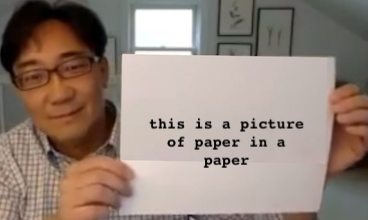
\includegraphics[width=0.7\columnwidth]{figs/figure}
\caption{
  The caption to this image.
  Make sure not to leave a blank line in here---LaTeX is dumb and will parse
  that incorrectly.
  %
  If you must, use a single percent sign to denote a blank line (see source
  file). The entire caption will still be rendered in a single paragraph.
}
\label{fig:example-fig-t}
\end{figure}

You can add figures at the top of the page, or inline. When specified with
\verb|[t]| option, images will be placed at the ``top''. Latex will figure where
``best'' to place the image, such as with Fig.~/ref{fig:example-fig-t}.
Make sure to include:
\begin{verbatim}
  \label{fig:example-fig}
\end{verbatim}
so that you can reference it with \verb|Fig.~\ref{fig:example-fig}|
and produce a linked reference like this Fig.~\ref{fig:example-fig-t}.
For these floating figures, also include \verb|\caption{the caption}| to add a
caption.

Otherwise, you can add figures inline using the \verb|center| environment:

\begin{center}
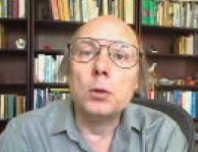
\includegraphics[width=0.3\columnwidth]{figs/figure2}
\end{center}

N.B. the tilde \verb|~| is an ``unsplittable'' space---it will never get
split across two different lines. This is useful before \verb|~\ref{...}|
and \verb|~\cite{...}|.

You need to add Bibtex references to \verb|references.bib|. Typical naming
convention is:
\begin{verbatim}
{Surname of first author}{Publication year}{First keyword of title}
\end{verbatim}
e.g. \verb|gu2015deep| for one of Ronghui's papers on deep specifications.
Then you can cite it with \verb|\cite{gu2015deep}|,
e.g.like this~\cite{gu2015deep}.
Make sure to use a \verb|~| before the citation.

I've defined a couple of comment macros in \verb|fastad-report.tex|.
\verb|\jhui{...}| will do this: \jhui{This is J-Hui's comment};
\verb|\jae{...}| will do this: \jae{This is James's comment}.
At the end, you can define these to become to be empty to quickly remove all
comments.
If you want to comment out a big block of text, just wrap them between
\verb|\if 0| and \verb|\fi|, like so (you cannot see what follows).
\if 0
C++ is not a programmer-friendly language.
\fi
